\section{Delving into Image Segmentation}

Image Segmentation is a fundamental concept in the realm of computer vision, which demonstrates how machines perceive and understand image data. The topic of \textbf{semantic segmentation} is the most essential part upnder this area. Semantic segmentation transcends the act of partitioning an image into various regions. It assigns each segmented region with a label, i.e. a \textbf{semantic meaning}, indicating what the region denotes. An illustrative example is provided in \autoref{fig:semantic-segmentation}, where the red region denotes the liver in a medical imaging scan. 

One worth mentioning is that semantic segmentation distinguishes itself from other tasks that merely cluster images into coherent regions, as shown in \autoref{fig:segmentations} \cite{segmentation-mli}. The regions identified through semantic segmentation carry a specific value or meaning inherently linked to the task at hand. In short, not just `where' but `what' is just as crucial in semantic segmentation.

\begin{figure}[htp]
    \centering
    \begin{subfigure}[b]{0.47\textwidth}
        \centering
        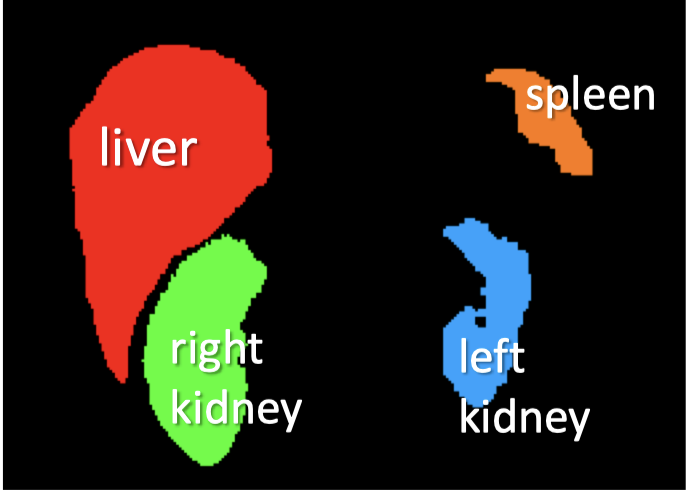
\includegraphics[width=\textwidth]{./figures/semantic-segmentation.png}
        \caption{Semantic Segementation}
        \label{fig:semantic-segmentation}
    \end{subfigure}
    \hfill
    \begin{subfigure}[b]{0.47\textwidth}
        \centering
        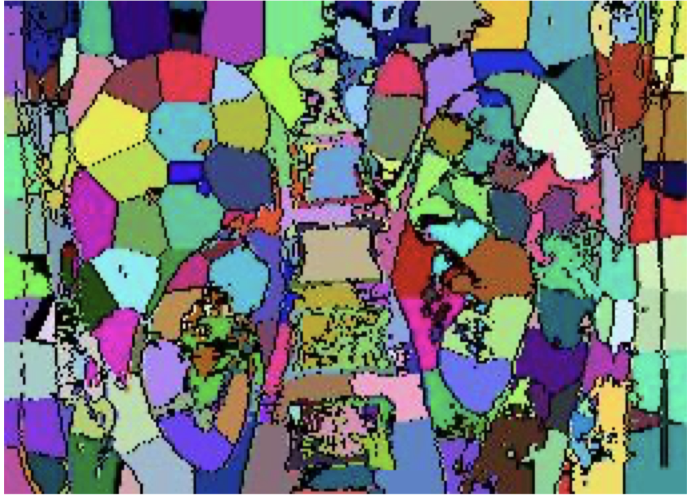
\includegraphics[width=\textwidth]{./figures/clustering.png}
        \caption{Segmentation based on clustering}
        \label{fig:normal-segmentation}
    \end{subfigure}
       \caption{Different Image Segmentation Tasks}
       \label{fig:segmentations}
\end{figure}

Having laid out an overview of semantic segmentation, we will delve deeper into the distinctive methodologies utilised for segmentation tasks in the following sections. This preliminary understanding provides a critical foundation for the exploration of more complex segmentation strategies and their applications in tasks such as diagnosing diseases or enhancing medical imaging methods.

\section{Manual Segmentation}
\label{sec:manual-segmentation}

Manual Segmentation, while basic, forms a cornerstone in the realm of image segmentation. In the context of our project, it involves utilising the specialised knowledge of medical experts to meticulously create `gold standard' labels for MRI data. This process requires careful slice-by-slice examination of the MRI data, highlighting the region of target organs, or the diseased from the healthy tissues. This level of detailed inspection ensures that such manual segmentation results in validated and trustworthy classifications.

However, manual segmentation does bring to light significant challenges. Notably, the time-intensive nature of this process becomes increasingly essential when dealing with large datasets. This situation is further compounded in scenarios requiring slice-by-slice analysis of MRI data. The resultant effect is that manual segmentation can be exceptionally time-consuming, limiting the volume of data that can be labelled within an acceptable timeframe.

This leads us to confront an ever-present challenge: the scarcity of gold standard labelled data. The considerable investment of time and skilled resources required for manual segmentation naturally restricts the availability of such high-quality, expert-classified data sets. As we journey towards leveraging machine learning methodologies in the realm of medical imaging, this scarcity of gold-standard, manually segmented data exerts a substantial hurdle to overcome. Thus, innovative solutions are required to address this gap and enhance the effectiveness and efficiency of image segmentation processes.

\section{Region-based Methods}
Region-based segmentation techniques, with the region-growing method standing as a prominent example, offer an alternative approach to image segmentation. This method hinges on the premise of homogeneity within the segmented regions. The algorithm initiates with a seed pixel and then expands the region by successively incorporating pixels similar to the initial seed. The process continues until the region growth reaches a pre-defined size or once the region achieves homogeneity, which is interpreted as the point when neighbouring pixels become significantly dissimilar \cite{adams1994seeded}.

The region growth method often proves effective because it generates a connected region starting from the seed point. Unlike thresholding methods that rely on explicit image properties, region-growing methods facilitate segmentation based on pixel similarity. However, this method exhibits sensitivity to noise, as the algorithm may persist in growing the region even if the neighbouring pixels significantly deviate from the seed pixel's properties.

Another key challenge when employing the region-growing method is the critical significance of the initial seed point selection. An incorrect choice of the seed point could obstruct proper region growth. This initial phase often becomes time-consuming and lacks accuracy when seeking the optimal seed point. Furthermore, it necessitates human intervention for evaluating the appropriateness of the chosen seed point.

\section{Deep Learning Methods}
\subsection{U-Net: An Automated Deep Learning Method for Image Segmentation}

U-Net \cite{ronneberger2015u} represents a transformative approach in the realm of deep learning methodologies for image segmentation. As an evolved variant of Fully Convolutional Networks (FCN) \cite{long2015fully}, U-Net integrates a high-level contextual extraction path with a symmetric localisation pathway. This unique arrangement both captures a broad context of the image and enables precise localisation of the targets. This is ideal for creating an automated pipeline for T.I. segmentations, and an essential requirement in our research. 

The end-to-end learning facilitated by U-Net directly generates pixel-wise segmentation masks from raw pixels, creating a valuable asset for our project. The architecture of this robust network is illustrated in \autoref{fig:unet}.

\begin{figure}[htp]
    \centering
    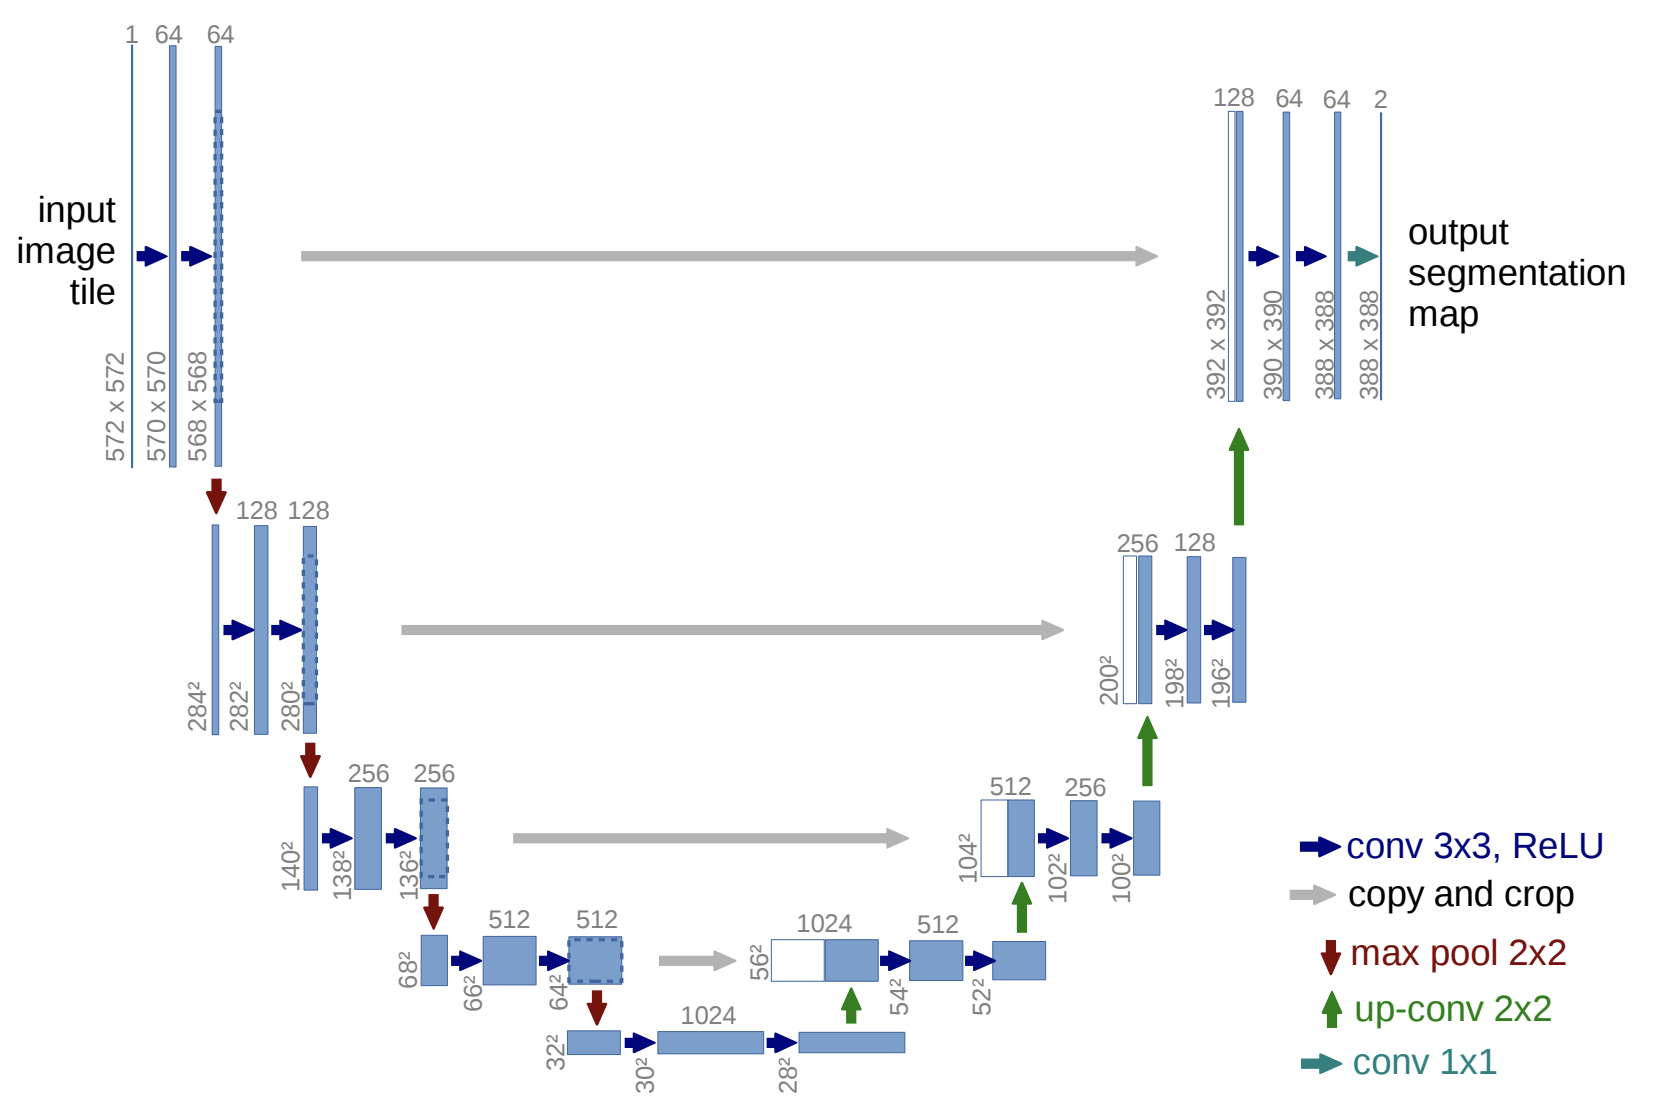
\includegraphics[width=\textwidth]{./figures/unet.png}
    \caption{An example of the U-net architecture.}
    \label{fig:unet}
\end{figure}

Significantly, U-net has also been developed to handle 3D data, which aligns perfectly with our scenario, where the MRI scans are inherently 3-dimensional images. Furthermore, each blue box in \autoref{fig:unet} encapsulates a multi-channel feature map. The number of channels is denoted at the top of each box, while the \(x\)-\(y\) dimensions are annotated at the lower left corner of the box. Meanwhile, the white boxes signify sets of copied feature maps, with arrows demonstrating varied operations.

On the contracting (left) side of the network, the design entails a series of recurrent steps. Each step initiates with two 3x3 convolutions, proceeding to double the number of feature maps. The result is then subjected to a Rectified Linear Unit (ReLU) activation function, followed by a downsampling operation using 2x2 max pooling with a stride of 2.

On the expansive side (right) of the network, the process commences with an upsampling step. A 2x2 convolution follows, halving the feature channels, which are then concatenated with their corresponding features from the contracting pathway. To conclude, a pair of 3x3 convolutions are applied to the image, succeeded by ReLU activations. The final layer employs a 1x1 convolution that maps each 64-component feature vector to the desired classes.

Overall, U-Net offers a comprehensive and highly effective tool for achieving granular image segmentation, which is indeed a capability integral to the success of our research exploration.

\subsection{nnU-Net: A Self-configuring Framework Aligned with Our Research Goals}
The nnU-Net \cite{isensee2021nnu} offers a progressive step towards personalised segmentation techniques. As a framework built upon U-Nets, it embodies a self-configuring segmentation mechanism, which autonomously orchestrates the configuration of preprocessing, network architecture, training, and post-processing steps in a segmentation pipeline. Crucially, the configuration selected is not static but instead adapts to the specificities of the medical data used for training. 

A standout feature of nnU-Net is its unique approach towards determining hyperparameters. The framework utilises “data fingerprints” allied with heuristic rules to pinpoint the optimal hyperparameter configuration for a given dataset before processing the training data. This data fingerprint concept is further leveraged to generate pipeline configurations, encapsulating both inferred parameters (such as image resampling, normalisation, batch, and patch size) and blueprint parameters (such as loss function, optimiser, and network architecture).

With these pre-selected hyperparameters and generated pipeline configurations, nnU-Net proceeds to facilitate network training for 2D, 3D full-resolution, and 3D-Cascade U-Nets \cite{isensee2018nnu}. The platform then select an ensemble of configurations from these three networks to achieve optimal performance (for instance, maximising the average dice coefficient). Once identified, this optimal configuration is subsequently deployed and evaluated on the test dataset.

\begin{figure}[htp]
    \centering
    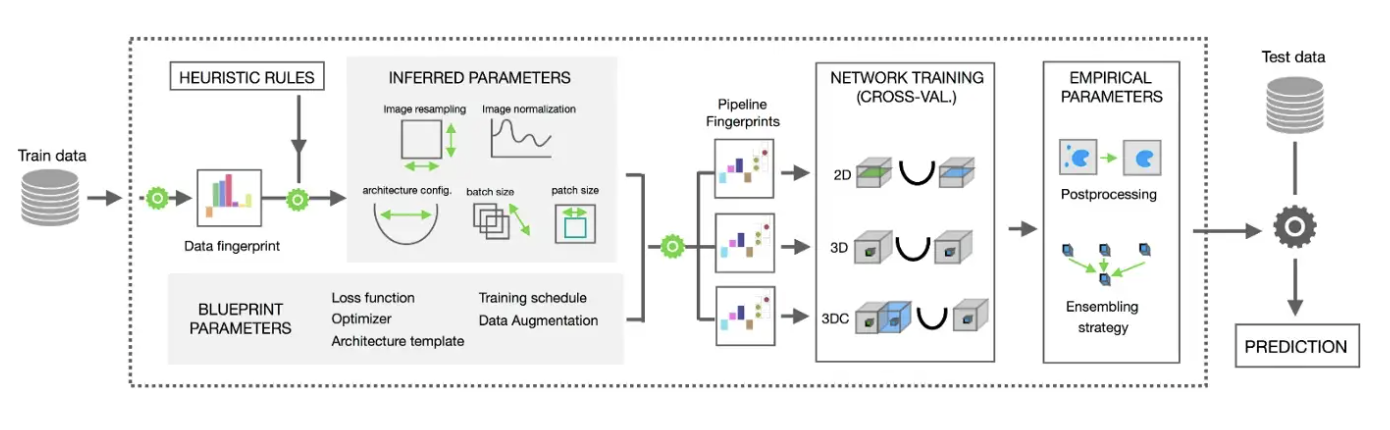
\includegraphics[width=\textwidth]{./figures/nnunet.png}
    \caption{The pipeline representation of nnU-Net.}
    \label{fig:nnu-net}
\end{figure}

Notably, nnU-Net has been shown to deliver state-of-the-art performance in various medical imaging tasks, including segmenting brain tumours, prostate tissues, and liver structures \cite{isensee2019nnu}.

Therefore, while nnU-Net enables a highly adaptive and automated segmentation workflow, the utility of the trained model is maximised when deployed on tasks that closely resemble the context and content of the training data. In our specific case, we will train the nnU-net model with our specific type of 3D MRI scans for T.I. segmentation tasks to ensure optimal results. This approach ensures leveraging the full potential of nnU-Net's adaptive capabilities tailored to our research goals.

As our research strives to establish an automated pipeline for T.I. segmentations on 3D MRI scans, integrating the nnU-Net framework is poignantly relevant. With its inherent capacity to adapt to different datasets and consistently yield precise image segmentation, nnU-Net is excellently positioned to enhance the rigour and precision of our research endeavour.

\section{Generating Weak Labels: A Strategic Response to Annotation Scarcity}

Given the scaricity of gold standard annotations for segmentation tasks, as discussed in \autoref{sec:manual-segmentation}, it becomes imperative to identify effective strategies that can enhance our training outcomes. One potential approach is the use of weak labels or weakly-segmented masks derived from the data. By adopting such methods, we aim to extract critical image features that can contribute to the learning efficacy of our model, despite limited access to manually-annotated, gold standard data.

\subsection{Leveraging Unsupervised Methods: Simple Linear Iterative Clustering (SLIC)}

Simple Linear Iterative Clustering (SLIC) \cite{achanta2010slic} is a notable unsupervised method we contemplate employing. This algorithm stands at the forefront of superpixel segmentation techniques, providing a powerful tool to cluster pixels within an image into compact and uniformly labelled regions, referred to as `superpixels'.

The key strengths of SLIC are its simplicity, ease of implementation, and adaptability across diverse scenarios. These virtues enable SLIC to handle boundary adherence issues effectively while reducing the computational burden associated with image segmentation tasks. Essentially, SLIC operates as a spatially constrained iterative k-means clustering method with a pre-determined superpixel. \autoref{fig:slic-example} shows an illustration of the effect using SLIC. 

\begin{figure}[htp]
    \centering
    \begin{subfigure}[b]{0.45\textwidth}
        \centering
        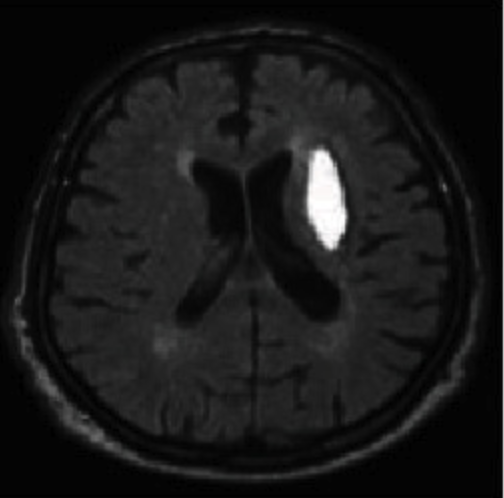
\includegraphics[width=0.8\textwidth]{./figures/slic-img.png}
        \caption{Original Image}
        \label{fig:slic-img}
    \end{subfigure}
    \hfill
    \begin{subfigure}[b]{0.45\textwidth}
        \centering
        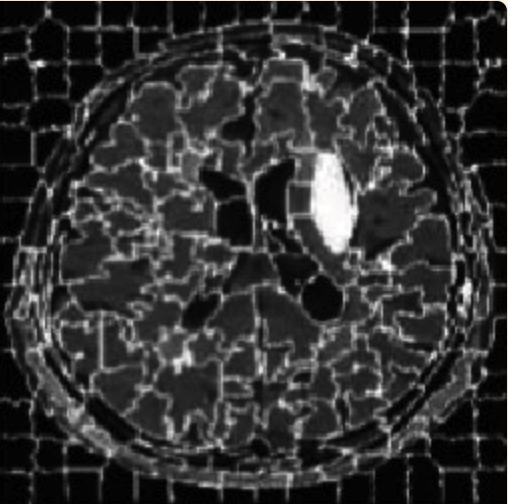
\includegraphics[width=0.8\textwidth]{./figures/slic-seg.png}
        \caption{Generated Superpixels}
        \label{fig:slic-seg}
    \end{subfigure}
    \caption{Superpixel Segementation using SLIC}
    \label{fig:slic-example}
\end{figure}

\begin{algorithm}[ht]
\caption{SLIC superpixel segmentation}\label{alg:slic}
\begin{algorithmic}[1]
\item Initialise cluster centers \(C_{k} = \left[l_{k}, a_{k}, b_{k}, x_{k}, y_{k}\right]^{\top}\) by sampling pixels at regular grid with grid intervel \(S\).
\item Perturb cluster centers in a \(n \times n\) neighbourhood, to the loweset gradient position.
\While{$E >$ threshold}
    \For{each cluster center \(C_{k}\)}
        \State {Assign the best matching pixels from a \(2S \times 2S\) square \newline
        \hspace*{3em}neighbourhood around the cluster according to \newline 
        \hspace*{3em}the distance measure \cite{achanta2010slic}.}
    \EndFor
    \State Compute new cluster centers and residual error \(E\).
\EndWhile
\item Enforce Connectivity.
\end{algorithmic}
\end{algorithm}

The SLIC algorithm adapted from \cite{achanta2010slic} is illustrated in \autoref{alg:slic}. Additionally, the residual error \(E\) in clustering is defined as the \(L_{1}\) distance between previous centers and recomputed centers.

By integrating SLIC as part of our weak label generation strategy, we aim to utilise these inherent benefits to enhance the robustness of our machine learning models, thereby bringing rich insights from our medical imaging data in the absence of extensive manually-curated annotations.

\subsection{Harnessing Pretrained Models: The Segment Anything Model (SAM)}
Emerging from the innovative approaches of Meta AI, the Segment Anything (SA) project presents a new paradigm for image segmentation. The cornerstone of this project is a pioneering model, known as SAM, which exhibits an impressive degree of adaptability and transferability. Specifically designed and trained to be promptable, SAM showcases remarkable capabilities in zero-shot transfer to new image distributions and tasks.

This inherent agility of SAM incites impressive zero-shot performance outcomes. Indeed, comparative analysis with prior fully supervised results reveals that SAM often delivers competitive, even superior, performance metrics \cite{kirillov2023segany}. Extending this versatile approach to medical imaging, MedSAM \cite{MedSAM} offers compelling prospects. Derived from the parent SAM model, MedSAM has shown considerable promise in segmenting medical images. One study unearthed that SAM's functionality can be enhanced with manual prompts, such as points and boxes, indicating intended objects in medical images \cite{huang2023segment}. This enhancement strategy aligns perfectly with our proposed approach to utilise the centerline coordinates and subsequently refine the segmentation process by obtaining finer-grained weak masks from SAM and MedSAM.

With its inspiring capabilities, the SAM model family holds immense potential to enhance our quest for automated and precision-driven segmentation techniques, thereby bolstering our research outcomes.












